\chapter{Monitoring WLCG with lambda-architecture} \label{lambda-eva}

%\section{Motivations} \label{Motivations}

\section{The evolution of WLCG activities monitoring} \label{lambda-intro}

Monitoring computing activities in the Worldwide LHC Computing Grid (WLCG)
\cite{wlcg}, such as job processing, data access and transfers or sites
availability, requires the gathering of monitoring data from
geographically-distributed sources and the processing of such information to
extract the relevant value for WLCG users, computing teams of the WLCG
organizations and WLCG site operators.  Current monitoring systems have proven to be
a solid and reliable solution to support WLCG functions and operations during
LHC data-taking years.  A variety of data coming from different services and
experiment-specific frameworks is gathered, processed and archived and a
generic web-based dashboard provides a uniform and customisable monitoring
interface for scientists and sites. Nevertheless, the current architecture,
where relational database systems are used to store, to process and to serve
monitoring data, has limitations in coping with the foreseen increase in the
volume (e.g.  higher LHC luminosity) and the variety (e.g. new data-transfer
protocols and new resource-types, such as cloud-computing) of WLCG monitoring
events. This paper presents the new data store and analytics platform which is
going to be used for the evolution of WLCG activities monitoring.

\subsection{WLCG data activities dashboards} 

The Experiment Dashboard (ED) \cite{Andreeva2009} is a generic monitoring
framework which provides uniform and customisable web-based interfaces for
scientists and sites. Monitoring events, such as data transfers or data
processing jobs reports, are collected and analysed to produce summary
time-series plots used by operators and experts to evaluate WLCG computing
activities. The WLCG Data acTivities (WDT) dashboards are a set of monitoring
tools based on the ED framework which are used to monitor data access and
transfer across WLCG sites via different protocols and services. Monitored
services include the ATLAS Distributed Data Manamegement (DDM) system, XRootD
and HTTP federations and the File Transfer Service (FTS).  The WDT use case is
one of the most data intensive ED applications. Figure \ref{fig:wdt} presents
the daily volume of monitoring information handled by WDT, with an overall
average of more than 20 million daily monitoring events.  Today, WDT
dashboards are suffering from the limitation of the current processing
infrastructure, as presented in the next section. For this reason, WDT is taken
as a case study for the new analytics platform.

% In the next future,
%the WLCG monitoring infrastructure have to cope with an extension of the volume
%(e.g. higher LHC luminosity) and the variety (e.g. new data-transfer protocols
%and new resource-types, as cloud-computing) of the monitoring data. 

%The task requires a sound knowledge of distributed systems theory and concepts together with a deep understanding of the new technology stack for large-scale data analysis. The project will be done relying on facilities and experience f%rom the Agile Monitoring initiative of the CERN IT department.

%The Experiment Dashboard (ref) is a generic web-based dashboard framework which is used to provide uniform and customisable monitoring interface for scientists and sites. The Figure in \ref{fig:wdtv} shows the daily volume of monitoring information processed by the different dashboards. While being a solid a reliable monitoring solution, the foreseen increase in data volume and variety of monitoring requires an evolution of the current archive and processing technology.   

\begin{figure}
  \centering
  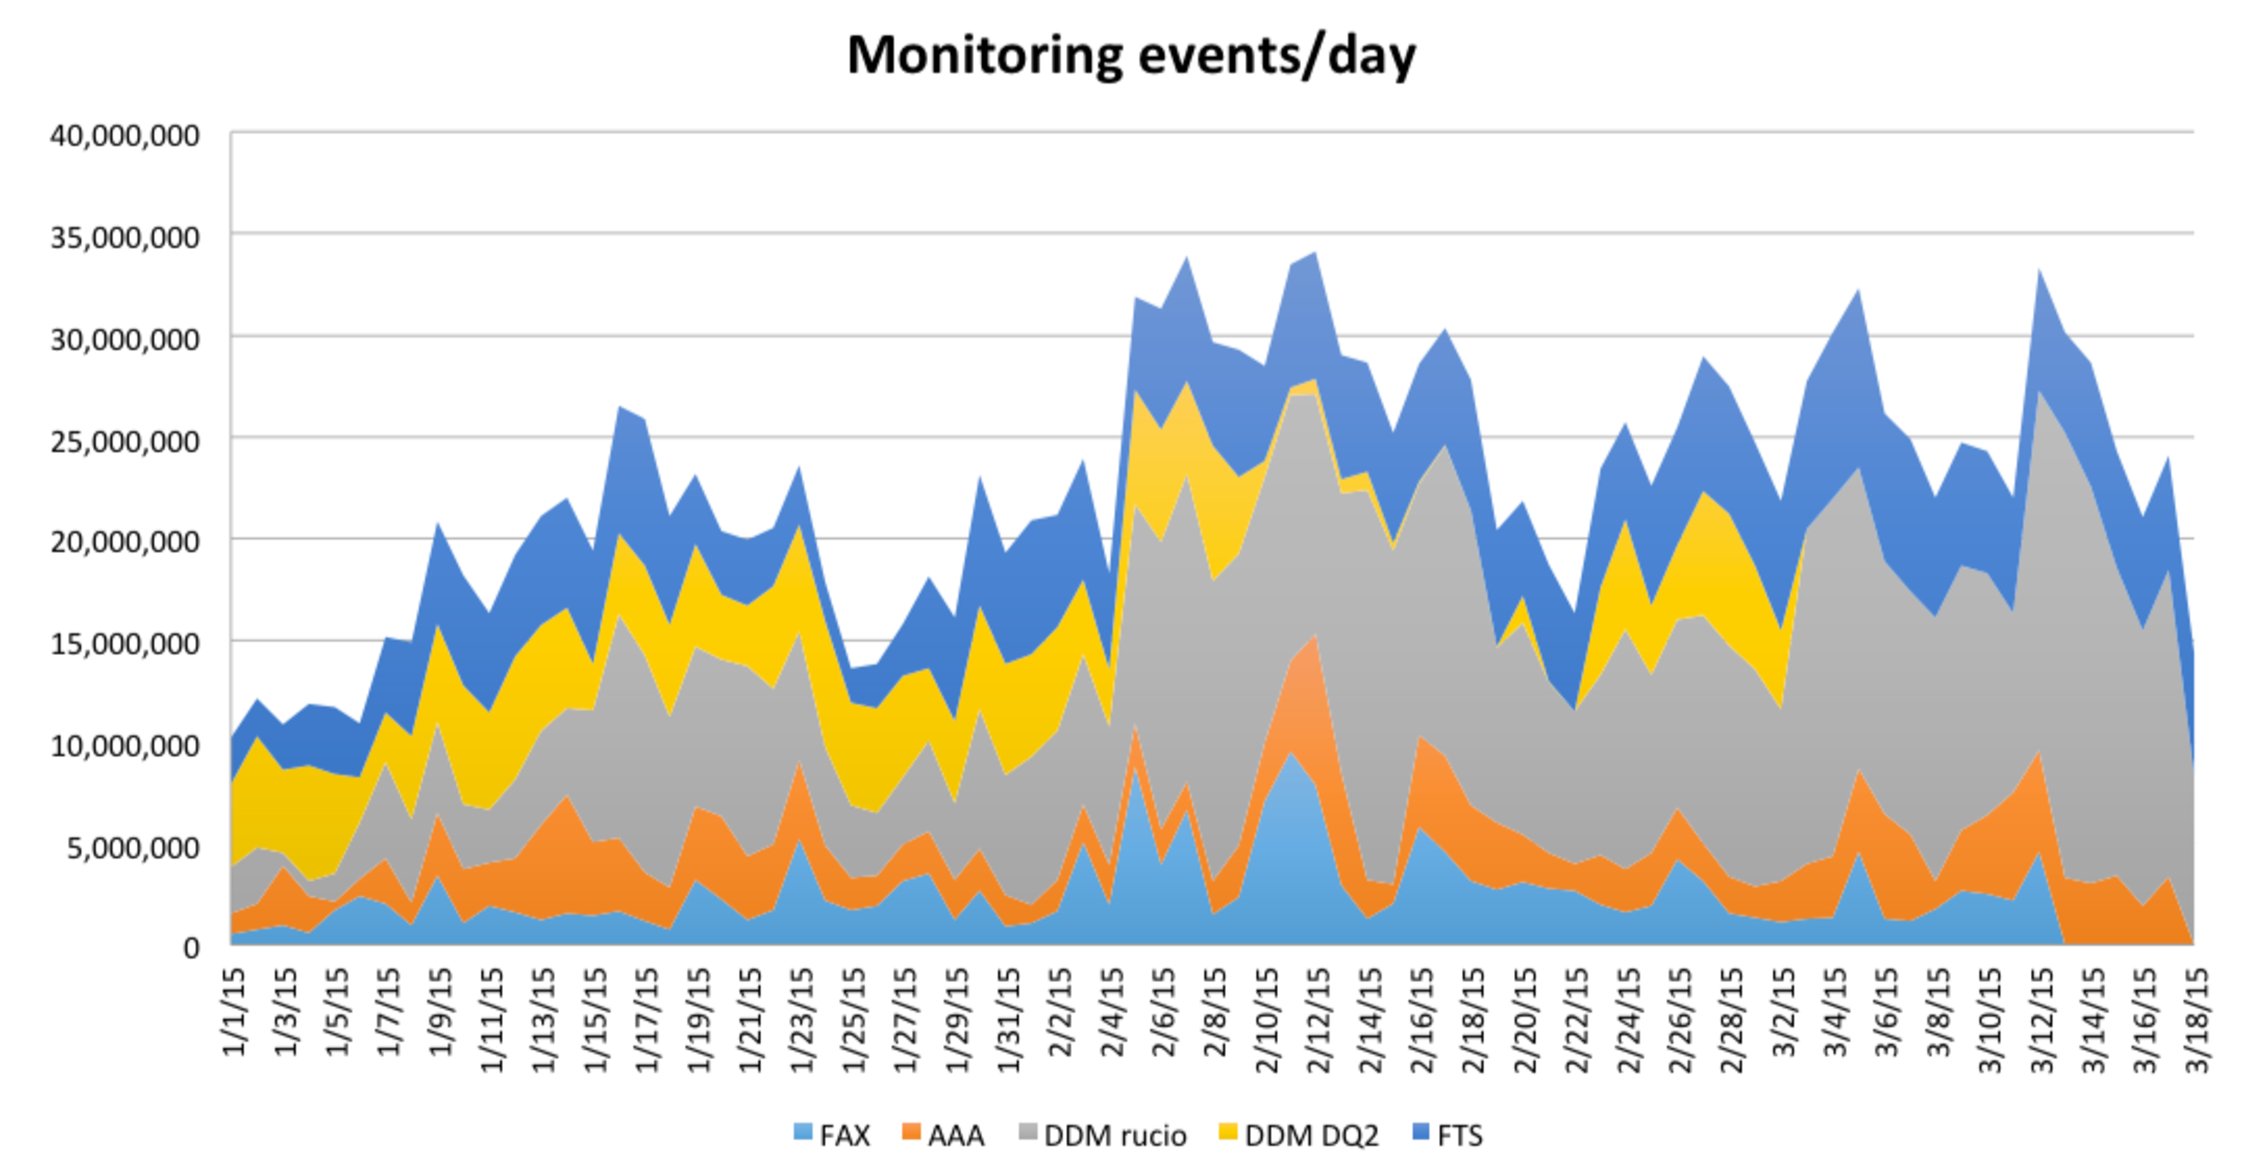
\includegraphics[width=120mm]{./Figures/wdt_volume.pdf}
  \caption{\small Daily volume of monitoring events for WDT dashboards.}\label{fig:wdt}
\end{figure}

\subsection{Towards a new approach for data store and processing} 

The current ED architecture relies on an Oracle database to store, to process
and to serve the monitoring data. Raw monitoring events are archived in tables
for several years, periodic PL/SQL jobs run at regular interval (10 minutes) to
transform the fresh raw data into summarized time-series statistics and feed
them in dedicated tables, from where they are exposed to the web-framework for
user visualization. For data intensive use cases, such as WDT, this approach
has several limitations. Scalability is difficult to achieve, PL/SQL execution
time fluctuating from tens of seconds to minutes as a consequence of the input
rate spikes, affecting user interface latency. Advanced processing algorithms
are complex to implement in PL/SQL within the dashboard 10 minutes time
constraint, and reprocessing of the full raw data can take days or weeks.
Moreover, the other dashboard components involved in data collection,
pre-processing and insertion are suffering from fragility and complexity,
leading to higher maintenance and operational costs and human faults.
Considering the foreseen increase in the WLCG monitoring data volume and
variety of monitoring events for the upcoming LHC runs, data store and
processing technologies which scale horizontally by design, such as Hadoop, are
suitable candidates for the evolution of the monitoring infrastructure. 
%The adoption of such technology requires a careful evaluation and the next
%sectiosn present the investiagtion done to esablish the best technology stack
%for the WLCG use case.
 

%\subsection{Requirements for the new architecture}

%The Monitoring section of the Support for Distributed Computing ( SDC) group, at the CERN IT department, is working on the research, the design and the development of the new data store and analytics platform for the evolution of the WLCG monitoring, able to cope with the scalability, flexibility and fault-tolerance requirements foreseen in the long-term WLCG scenario. 


%Requirements: Scalability/Simplicity/Mainstream

\section{The \textit{lambda} architecture}

In recent years, the challenge of handling a big volume of data has been taken
on by many companies, particularly in the internet domain, leading to a full
paradigm shift on data archiving, processing and visualisation. A number of new
technologies have appeared, each one targeting specific aspects on big-scale
distributed data-processing. All these technologies, such as batch
computation systems (e.g. Hadoop) and non-structured databases, can handle very
large data volumes with little cost but with serious trade-offs. The goal is to
architect a new platform in a tool-chain approach building on the most
appropriate technologies and computing techniques for the WLCG use case.

In this direction, the lambda architecture, presented by Marz in \cite{lambda} and successfully adopted by companies such as Twitter for data analysis, identified 3 main components to build a scalable and reliable data processing system:
\begin{itemize}
\item  the \textbf{batch layer}, to store a steadily growing dataset providing the ability to compute arbitrary functions on it;
\item  the \textbf{serving layer}, to save the processed views, using indexing techniques to make them efficiently query-able;
\item  the \textbf{real-time layer} able to perform analytics on fresh data with incremental algorithms to compensate for batch-processing latency. 
%Moreover, the real-time analytics layer can be used as input for active-reaction, adopting classical pattern matching approach to detecting errors and failures on the stream of monitoring events promptly. 
\end{itemize}

%\begin{figure}
%  \centering
%  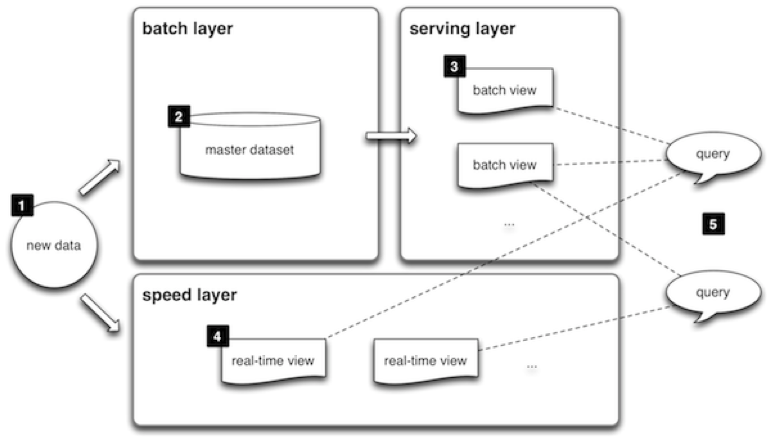
\includegraphics[width=60mm]{./Figures/lambda.png}
%  \caption{\small Sketch of the Lambda architecture, from (ref).}\label{fig:Lambda}
%\end{figure}

\subsection{Difference between WDT and the classic lambda use case}

In the classic lambda application each monitoring event only contributes to the
most recent view (e.g. a web server user access for a web analytics application
only affects the user count in the last time bin). For the WLCG monitoring use
case, this is not true. A monitoring event, such as a completed file transfer
lasting several hours from WLCG site A to site B, contributes also to several
time bins in the past, so that the information about the average traffic from
site A to site B has to be updated accordingly with the new monitoring
information. Without this initial hypothesis, the merging of batch and
real-time processing becomes more complex, as discussed in section 3.

\section{The new data store and analytics platform for WLCG monitoring}

The new data store and analytics platform for WLCG monitoring is presented in
Figure \ref{fig:narch} and it builds on a number of existing technologies and
tools in order to promote mainstream solutions and to minimize in-house code
development. The WLCG monitoring problem has been treated as a pure analytics
scenario where the driving concepts, as by the lambda principles, are to
collect and to store the raw data, to minimize pre-processing and to concentrate
analysis and transformation on the same framework with batch and real-time
components. 

\begin{figure}
  \centering
  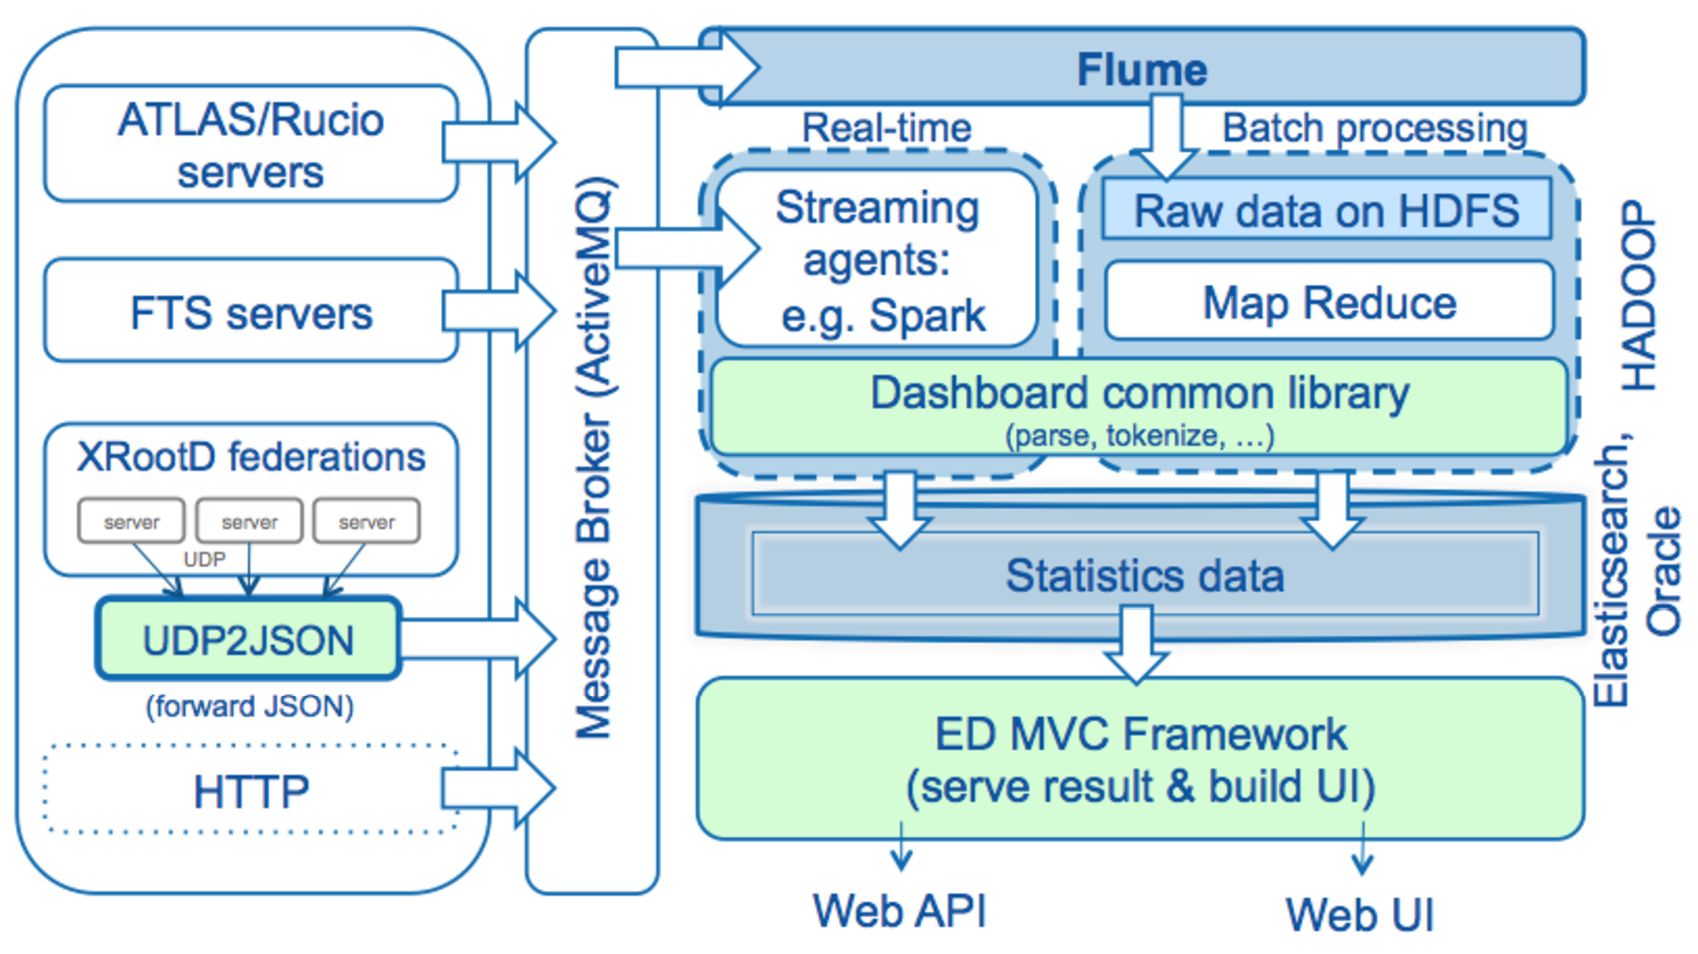
\includegraphics[width=120mm]{./Figures/new_arch.pdf}
  \caption{\small The new data analytics platform for WLCG monitoring.}\label{fig:narch}
\end{figure}

\subsection{Data transport: Message Broker}

The transport layer plays a key role in the new monitoring architecture.
Firstly, it decouples the producer and the consumer of the monitoring data.
Given that the information is produced by a variety of heterogeneous
applications and services in WLCG, this is a fundamental part of the system
functionality. Secondly, it allows multiple consumers to use the same data via
on-demand public/subscribe API. This situation is often the case for monitoring
data, which is also being used by LHC experiment specific frameworks. Thirdly,
the architecture can rely on message brokers as a service provided by the CERN
IT infrastructure. Currently, the broker technology used is ActiveMQ and the
monitoring events are reported as JSON records via the STOMP protocol.  A
possible future evolution is to explore tools such as Apache Kafka, a
specialized broker which improves the handling of big data volumes and works at
a higher data rate.

\subsection{Data collection: Apache Flume}

Apache Flume is used as the data collector agent. It receives monitoring events
from the transport layer and creates HDFS files in the archive layer for later
processing. It replaces a custom collector previously developed for the ED
framework, providing better performance and reliability. Flume connects to the
brokers using the standard JMS source and writes to the storage layer via the
standard HDFS sink.

\subsection{Batch processing: Apache Hadoop}

Hadoop is a distributed processing framework which allows the computation of
large data sets on computer clusters built from commodity hardware. Initially
focused mainly on batch-processing via the MapReduce primitives
\cite{mrgoogle}, modern Hadoop supports multiple processing technology, such as
Apache Spark.  MapReduce is the de-facto standard for batch processing and its
computation paradigm fits extremely well with the WDT use case, as presented in
section 4.  WDT batch-processing is implemented as periodic MapReduce jobs
running on the Hadoop infrastructure provided from CERN IT. The job algorithm
is stateless and idempotent, the full data set which can contribute to the
results (e.g. 3 days of data) being re-processed at each run. Job results are
written into the serving layer (i.e. Oracle table), which is then used to build
the web visualization. Moreover, WDT jobs also support Apache Spark
\cite{spark} as a processing framework. Spark is a modern distributed processing
technology, running on Hadoop or on standalone clusters, which improves the
MapReduce paradigm with a better in-memory computational model. In addition, it
also supports data streaming, which is useful in a lambda architecture to limit
code differences between batch and real-time. This flexibility is achieved via
the common WDT library presented below, which abstracts shared functionalities
and algorithms.


\subsection{Real-time processing: Spark streaming and Esper} 

Spark provides a streaming API for distributed processing of event streams.  A
continuous flow of data is divided into micro-batches (e.g. 10 seconds of events)
which can then be processed as if they were local data sets via standard Spark
in-memory primitives. Spark streaming jobs have been implemented to compute WDT
statistics on fresh monitoring events via an incremental algorithm.  Being
incremental hence not idempotent, special care is required in handling event
duplication and multiple processing, leading to a more error prone computation.
For this reason, and as by the lambda principles, the results from the
streaming jobs are continuously overwritten by the batch processing at each run
(e.g. every hour). Moreover, WDT streaming jobs were also implemented using
the open source event processing library Esper \cite{esper}. Compared with the basic Spark
primitives, Esper SQL-like language offers much more advanced controls in
processing streams over time.  For the WDT use case, where a basic map/reduce
paradigm fits the algorithm, the raw Spark primitives were preferred, but Esper
remains a valid option for other WLCG monitoring use cases when more advanced
processing is required. A possible evolution in this direction is to
investigate Esper as an embedded Spark streaming operator.
 

\subsection{Archiving: HDFS} 

The Hadoop framework is built on the Hadoop Distributed File System (HDFS) and
executes I/O operations on it. HDFS is designed for large data files, in the
order of GigaBytes in size. The data is broken into blocks and replicated
across multiple hosts in the cluster. This guarantees scalability on commodity
hardware, fault tolerance and high throughput. HDFS is data format independent,
it supports multiple data representations, from simple text to structured
binary. Section 4 presents the data format evaluation performed for the WDT use
case.

\subsection{The Dashboard Common library}
A common drawback of the dual processing nature of the lambda architecture is the
code duplication in the real-time and the batch processing layer. In order to
limit this effect a Java library has been developed to abstract the
common functionalities for the WDT use case. The library provides data parsing,
supporting marshalling and un-marshalling in several formats, such as JSON, CSV,
Avro, and also provides data validation and compression. Most importantly, it implements
the algorithm to emit key-value pairs for each monitoring events received. The
library played a major role in porting the WDT jobs to different processing
technologies (e.g. MapReduce, Spark) with minimal code change.

\subsection{The serving layer}

With the data archiving and processing delegated to the other components,
the serving layer is solely responsible for serving the computed statistics to
the ED web framework. In light of this simplified
requirement, for the WDT use case the serving layer can be easily implemented
via relational databases as well as by non-relational technology. In the new data analytics platform
the serving layer is still implemented using an Oracle database provided from
CERN IT database service. A promising investigation, still ongoing, is pointing at
Elasticsearch as a particularly good candidate to replace the current database.

\section{Implementation of WDT analytics on the new platform}
 
The current architecture uses PL/SQL procedures for aggregating and computing raw data into statistics with different time period granularities and stores them into a statistics table. WLCG data servers can produce monitoring logs at 1 kHz, with such a rate that the PL/SQL procedure cannot cope with the overwhelming amount of data, which takes over ten minutes to process every ten minutes worth of data. The new analytics platform relies on Hadoop and its MapReduce framework to overcome the current latency and scalability issues. MapReduce is a programming paradigm that was designed to remove the complexity of processing data that are geographically scattered around a distributed infrastructure \cite{mrgoogle}. It hides the complexity of computing in parallel, load balancing and fault tolerance over an extensive range of interconnected machines. There are two simple parallel methods, \textit{map} and \textit{reduce}, which are predefined in the MapReduce programming model and are user-specified methods that are used to develop the analytics platform.

%\par


\begin{figure}
  \centering
  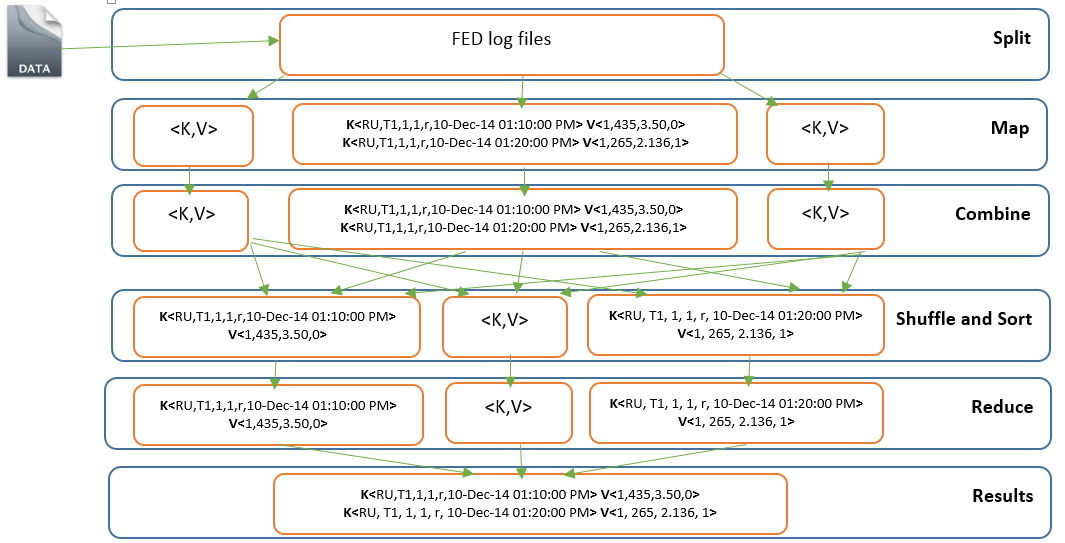
\includegraphics[width=100mm]{./Figures/MR.png}
  \caption{\small MapReduce computations diagram.}\label{fig:mapframe}
\end{figure}

\vspace{5mm}

Figure \ref{fig:mapframe} shows an how WDT MapReduce jobs are carried out by each component within the MapReduce framework: 

\begin{enumerate}
 \item A \textit{splitter} will split the monitoring data into lines and feed them into mappers.
 \item A \textit{mapper} will process the line; breaking them into the time bins in which they belong and calculating the transfer matrices. %(e.g. transferred bytes, active files, finished files, active time, etc.). 
Finally, it will emit key/value pairs for each time bin.
 \item A \textit{combiner} will run after each map task and aggregate a map output result, decreasing the number of metrics sent to the reducer.
 \item The output of the combiner is then shuffled and transferred to a reducer that is responsible for processing the key  and carrying out the final summing.
 \item A \textit{reducer} will aggregate and output the final results.
\end{enumerate}

\subsection{Data representation}
In the current architecture the data are partitioned in HDFS, as shown in Figure \ref{fig:dstructure}, for efficient processing, as this will support the processing of data by specified date ranges.

\begin{figure}[!htb]
\centering
\begin{minipage}{.5\textwidth}
\centering
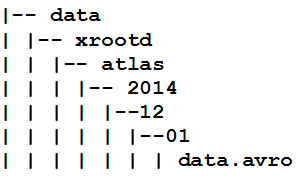
\includegraphics[width=60mm]{./Figures/dstructure.png}
\caption{\small HDFS data partitioning.}\label{fig:dstructure}
\end{minipage}%
\begin{minipage}{0.5\textwidth}
\centering
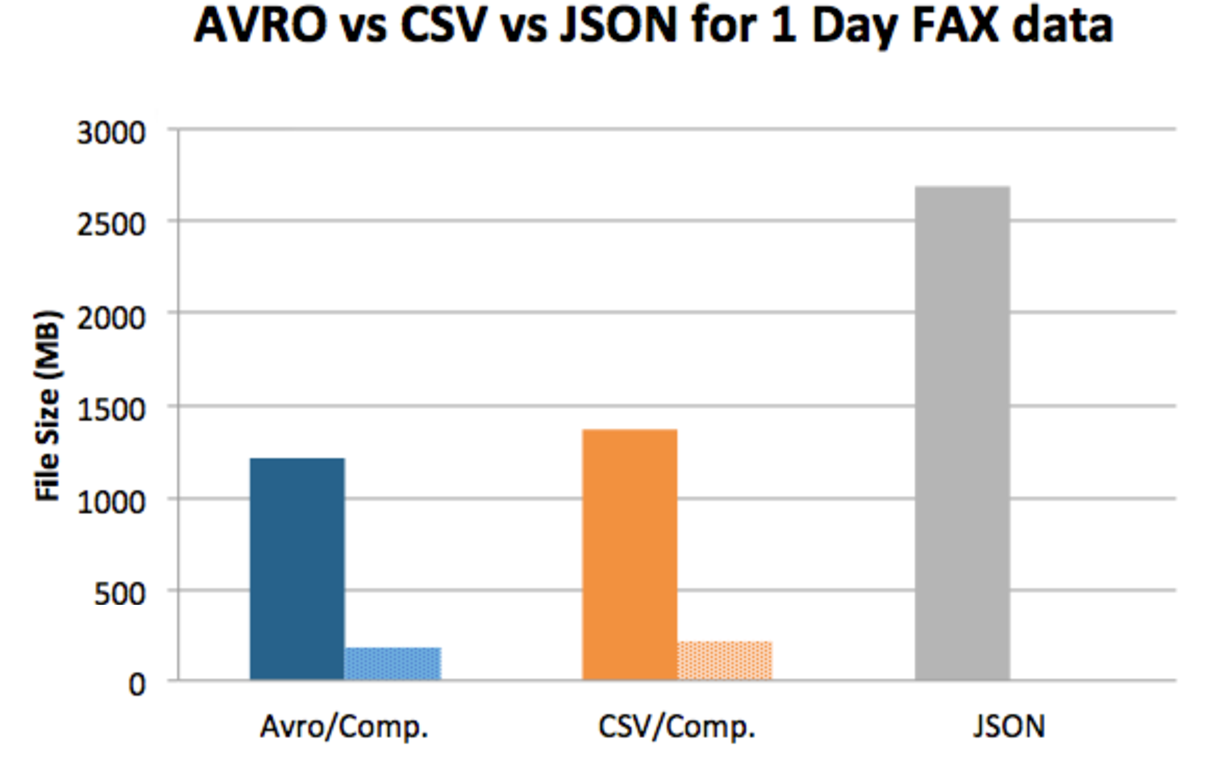
\includegraphics[width=60mm]{./Figures/format_plot.pdf}
\caption{\small Data format comparison.}\label{fig:format}
\end{minipage}
\end{figure}

Three different data formats were evaluated to store WDT monitoring data on HDFS: 
\begin{enumerate}
\item Avro is a data serialisation framework that serialises the data into a compact binary format, so that it can be transferred efficiently across the network.
\item Comma-Separated Value (CSV) is a table format that maps very well to the tabular data.
\item JavaScript Object Notation (JSON) is primarily a way to store simple object trees.
\end{enumerate}
\vspace{5mm}
Figure \ref{fig:format} shows data representing 1 (average) day of monitoring events for the ATLAS XRootD federation (FAX) on HDFS which occupies 1211 MBytes in Avro, 1367 MBytes in CSV and 2669 MBytes in JSON file format. 
%Figure \ref{fig:format} shows one day of data collected from the ATLAS XRootD federation (FAX), which clusters Tier-1, Tier-2 and Tier-3 storage resources together into a common namespace and allows remote accessibility from geographically separated sites
As expected, the Avro format is more compact than CSV and JSON. This is because the binary version of Avro is used, whereas CSV comprises human readable comma-separated columns and JSON contains tree structured data. The JSON format took a larger space because it holds both column name and data, whereas CSV only holds the data that are separated by comma. This has resulted in a 122.21\% increase in volume for JSON data and a 12.88\% increase in volume for CSV data compared with Avro, while there is a 96.85\% increase in volume for JSON data compared with CSV. The data were also compressed using the Snappy compression library, which is very fast but the compaction ratio is very low compared with other libraries. Again, compressed Avro data takes up much less room than the CSV as there is a 20.90\% increase in volume. It can be seen that compressed data took over 5 times less space than uncompressed. The test results, combined with the additional benefits of being schema-based and its multi-language support, make Avro the preferred option for the WDT use case.  
%\begin{figure}
 % \centering
 % 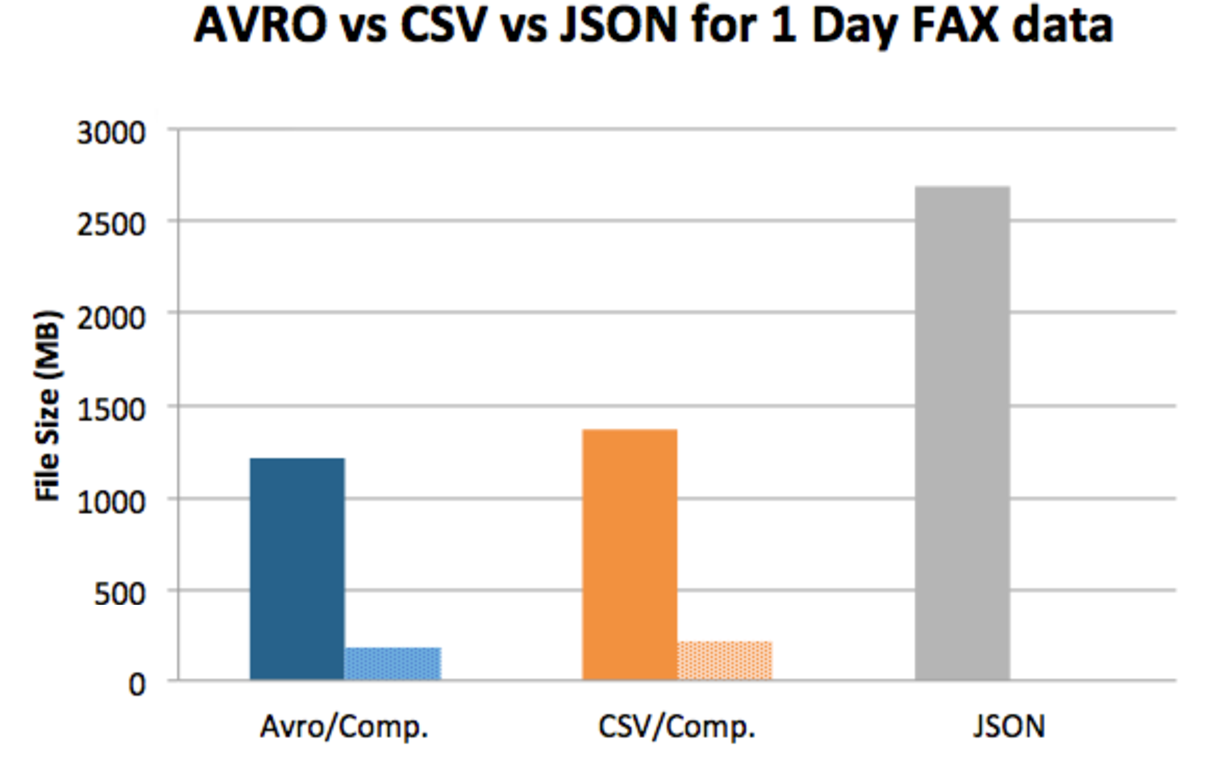
\includegraphics[width=60mm]{./Figures/format_plot.pdf}
 % \caption{\small Data format comparison.}\label{fig:format}
%\end{figure}

\section{Performance results for WDT computation on the new platform}
%Avro, CSV , JSON
%Partitioning
In order to evaluate the execution time of jobs on the new platform architecture, it was decided to compute FAX dataset by days, ranging from: 1 day, 3 days, 7 days and 21 days. Jobs were submitted a few times for each dataset  in order to capture an average performance time. The performance measurements were carried out on a heterogeneous Hadoop cluster that consisted of fifteen nodes (8 nodes: 32 cores/64GB, 7 nodes: 4 cores/8GB).

%and their specifications were as shown in Table \ref{table:1}.

%\begin{table}[h!]
%\centering
%\caption{Cluster specifications}
%\begin{tabular}{ l | c }
%  \hline  
%	 No.Nodes & Specifications \\ \hline
%  8 nodes & 32 cores/64GB \\
%  7 nodes & 4 cores/8GB  \\
%  \hline  
%\end{tabular}
%\label{table:1}
%\end{table}
The main result, as presented by the plot in Figure \ref{fig:mr}, is that the jobs were able to successfully process all data ranges in at most just few minutes. This result alone satisfies the WDT requirement of updating monitoring information every 10 minutes with fresh data and allows for re-processing of years of monitoring logs. Moreover, it demonstrates the scalability of the system over different data volumes.
%In Figure \ref{fig:mr}, the comparison between the execution time and data input size of compressed and uncompressed Avro, CSV and JSON jobs can be seen. 
In general, computation of uncompressed data was faster than compressed data with the exception of JSON data as it is very large compared to other formats. It is understandable why compressed data were slow to process as the data will need to be uncompressed before processing and will therefore add additional overheads to the computation time. Although uncompressed Avro and CSV jobs were fast, the CSV appears to be the fastest.
% This observation contradicted previous experiments conducted on another cluster as Avro clearly outperformed the CSV in this earlier study. 
This can be explained by the computing limitation of the cluster due to its heterogeneous setup.
%  It was expected that the processing time for CSV data would be longer than for Avro data because use of CSV format adds an extra overhead for parsing data into appropriate data types for computations, whereas Avro is not required to parse data due to the fact that data are accompanied with a schema. However, this was found not to be the case on this cluster and the logical explanation is that the nodes are unbalanced as 8 of the total 15 nodes have a high specification and 7 are average. Therefore, CSV data could have been distributed to the high performance nodes, whereas the Avro data could have been delivered to the average nodes, resulting in the parsing and computing of CSV data at a faster speed than for the Avro data.

It should be noted that largely there is not much difference between the execution time of the process on the 1 day dataset compared with the 21 day dataset, while being many times bigger in size. This demonstrates the scalability of the Hadoop system, which distributes the computation across several nodes. Nevertheless, there is always a fixed overhead added to the job for finding appropriate resources and submitting them. Even though the job is split into multiple map tasks and sent to data nodes where the data reside in order to reduce the movement of large data files over the network, the intermediate results of these tasks still need to be shuffled and shifted around to reducers (most likely to different nodes) \cite{mrgoogle}. This could create a bottleneck in the network, so in order to minimise this issue, it was decided to compress the intermediate results, improving by $\sim2$ seconds the time for transferring them to the reducer nodes. This results were obtained using the MapReduce version of the WDT jobs, but comparable measurements have been observed using Apache Spark for batch processing.

%\subsection{MR performance}
\begin{figure}
  \centering
  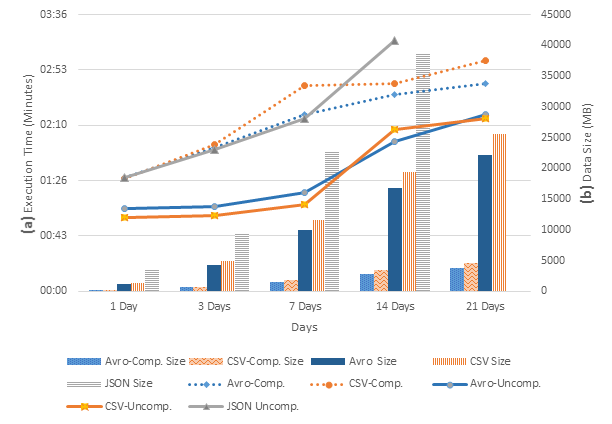
\includegraphics[width=140mm,height=80mm]{./Figures/mp_perf.png}
  \caption{\small Computation of Compressed/Uncompressed Avro, CSV and JSON files over different date ranges. The primary axis (a) shows the execution time that is being represented by lines, whereas the secondary axis (b) represents the input data size in Megabytes (MB) which is represented by bars.}\label{fig:mr}
\end{figure}

\section{Conclusion and next steps}

The new data store and analytics platform presented in this paper is a
scalable, simplified and effective solution for WLCG activities monitoring. It
builds on a set of mainstream technologies, and uses the lambda architecture
principles to assemble them in a reliable and effective way. The performance
test results show how the MapReduce/Spark approach outperforms the current
system and that it can scale horizontally to support the increase of the
volume and the variety of WLCG monitoring events in the upcoming years of LHC data
taking.

The next steps are to complete the migration of the WDT dashboards to the new
architecture and to evaluate the new platform for the other Experiment
Dashboard applications. Further investigation into the serving layer technology
and the optimal strategy for integrating batch and real-time data processing is
ongoing. 




